% !TeX document-id = {55cdd1f2-c708-43a6-9dcf-ca7bc9e91f17}
% !BIB program = biber
\documentclass[10pt]{beamer}

\usetheme{scilifelab}
\usepackage{appendixnumberbeamer}

\usepackage{booktabs}
\usepackage[scale=2]{ccicons}

\usepackage{hyperref}
\hypersetup{colorlinks=true, linkcolor=scAqua, urlcolor=scAqua, citecolor=scAqua}

\usepackage[backend=biber,style=apa, sortcites=true,sorting=nyt]{biblatex}
\addbibresource{literature/base-odyssey.bib}


\usepackage{pgfplots}
\usepgfplotslibrary{dateplot}

\usepackage{xspace}
\newcommand{\themename}{\textbf{\textsc{scilifelab}}\xspace}
\newcommand{\credit}[1]{{\vspace{\fill} \par \raggedleft \scriptsize \mdseries \color{mDarkBrown} #1 \par}}
\newcommand{\creditdark}[1]{{\vspace{\fill} \par \raggedleft \scriptsize \mdseries \color{scMGray} #1 \par}}
\newcommand{\creditdarknofill}[1]{{\par \raggedleft \scriptsize \mdseries \color{scMGray} #1 \par}}
\newcommand{\creditleft}[1]{{\vspace{\fill} \par \raggedright \scriptsize \mdseries \color{mDarkBrown} #1 \par}}
\newcommand{\creditdarkleft}[1]{{\vspace{\fill} \par \raggedright \scriptsize \mdseries \color{scMGray} #1 \par}}
\newcommand{\creditdarkleftnofill}[1]{{\par \raggedright \scriptsize \mdseries \color{scMGray} #1 \par}}
\newcommand{\citeme}[1]{{\xspace\color{scAqua} \scriptsize [\cite{#1}]}}
\newcommand{\feature}[1]{{\color{scLime} \textbf{#1}}}
\newcommand{\remark}[1]{{\par \color{scGrape} \ensuremath{\rightarrow} \emph{#1}}}

\makeatletter
\newcommand*{\myroman}[1]{{\fontfamily{ptm}\selectfont \expandafter\@slowromancap\romannumeral #1@}}
\makeatother

\title{2001: A Base Odyssey}
\subtitle{The era of genomics and massive parallel sequencing}
\date{February 24, 2025}
\author{Matthias Zepper, PhD}
\institute{NGI Stockholm\par \href{https://ngisweden.scilifelab.se}{https://ngisweden.scilifelab.se}}
\titlegraphic{\hfill
\includegraphics[height=1cm]{./additional_graphics/SciLifeLab_Logotype_Green_POS.png}}

\begin{document}

\maketitle

\begin{frame}{2001: Draft assemblies of the human genome are published}
	\begin{figure}
		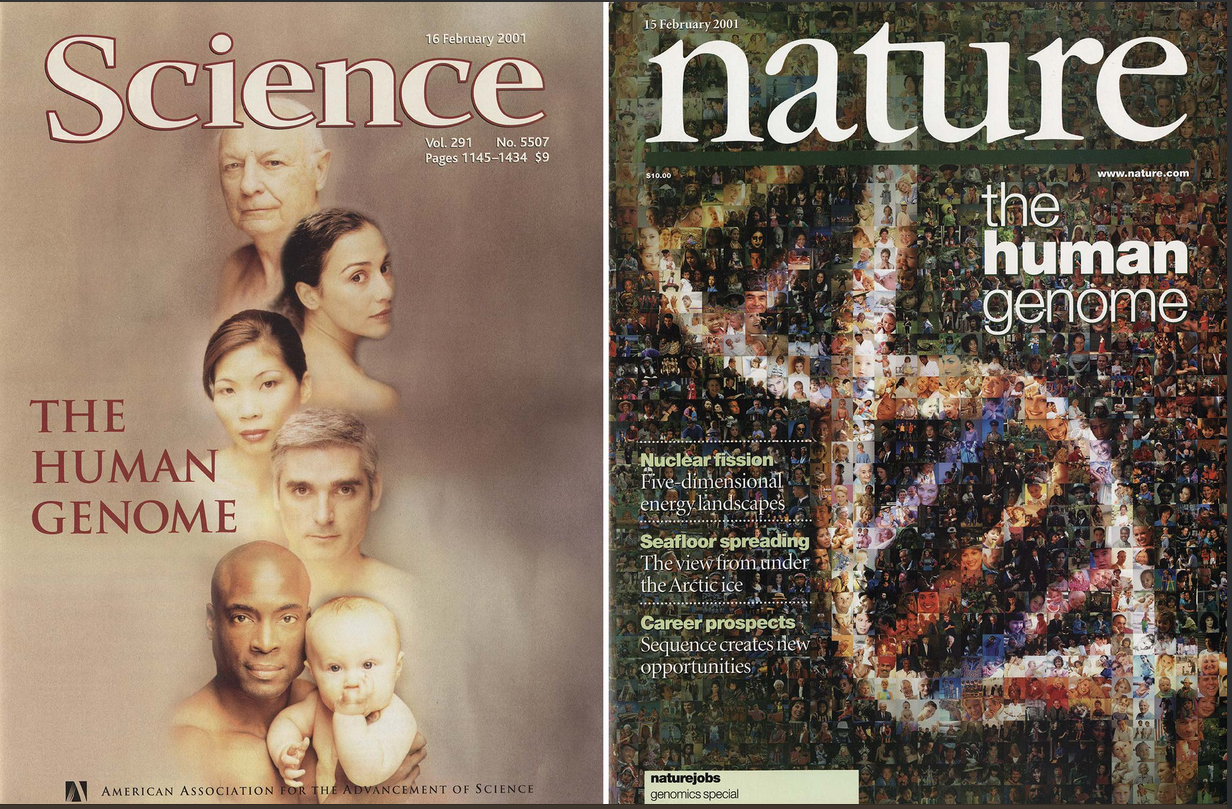
\includegraphics[width=0.8\textwidth]{figures/humangenomeproject.png}
		\caption{The private company Celera\citeme{Venter2001} and the International Human Genome Sequencing Consortium\citeme{Lander2001} both publish a draft sequence of the euchromatic portion of the human genome.}
	\end{figure}
	\credit{doi: 10.1126/science.1058040; doi: 10.1038/35057062}
\end{frame}

\begin{frame}[standout]{The overture to the genomic era}
	\begin{figure}
		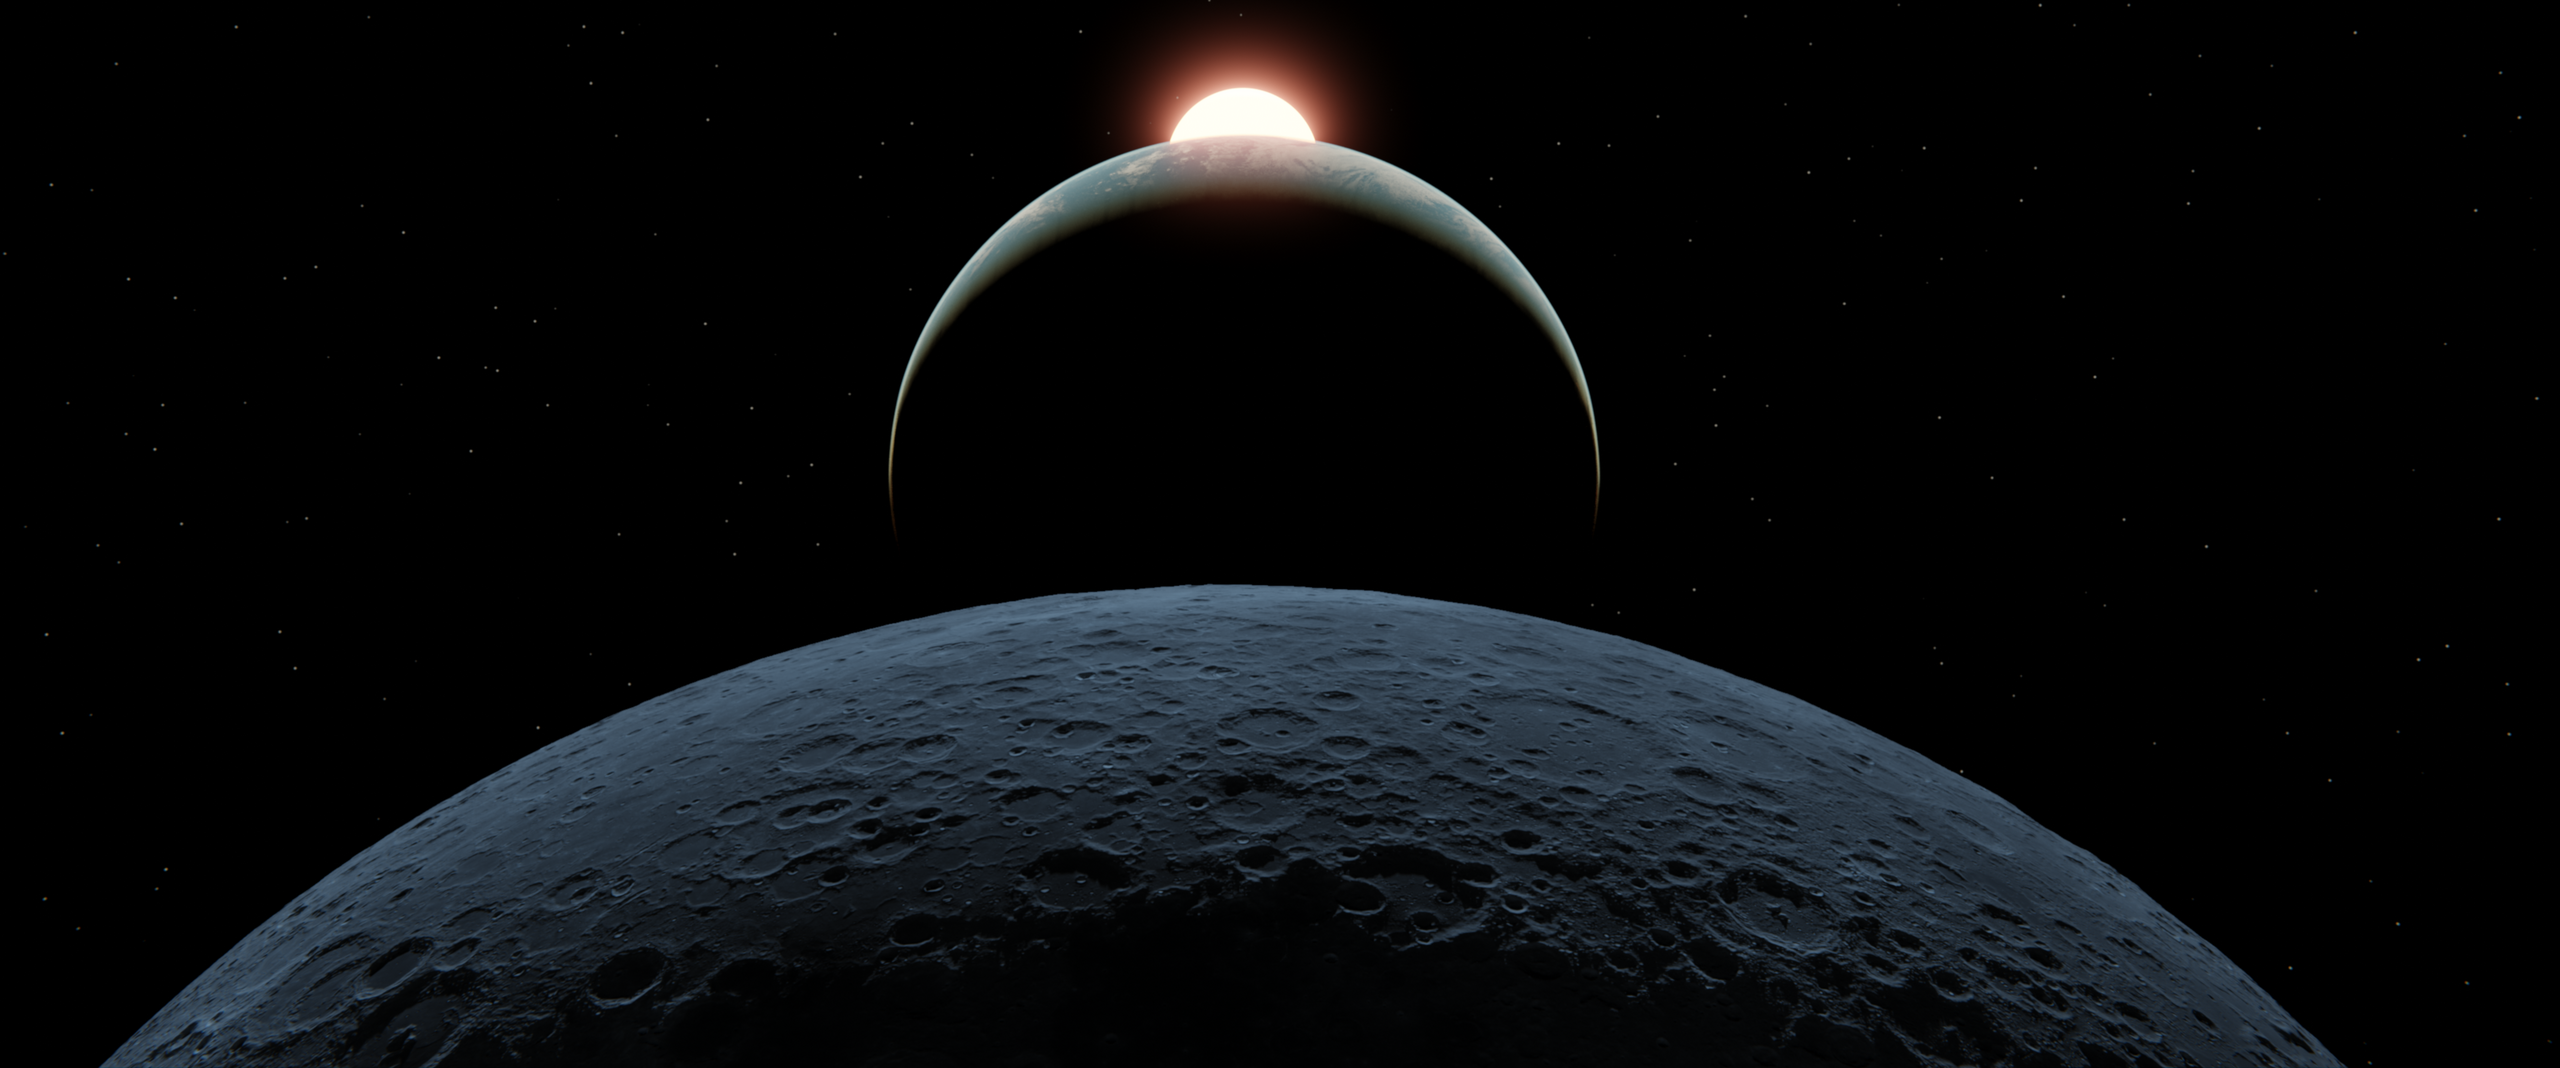
\includegraphics[width=\textwidth]{./additional_graphics/Opening_2001-_A_Space_Odyssey.png}
		\creditdarknofill{A remake of the opening scene by SumoSebi, \href{https://commons.wikimedia.org/wiki/File:Opening_2001-_A_Space_Odyssey.png}{CC-BY-SA on Wikimedia Commons}}
	\end{figure}
	{\small	Stanley Kubrick's \emph{2001- A Space Odyssey} premieres  2 April 1968}

\end{frame}

\begin{frame}{1968: Nobel prize for the interpretation of the genetic code}
	\begin{columns}[T,onlytextwidth]
		\column{0.6\textwidth}
		\begin{figure}
			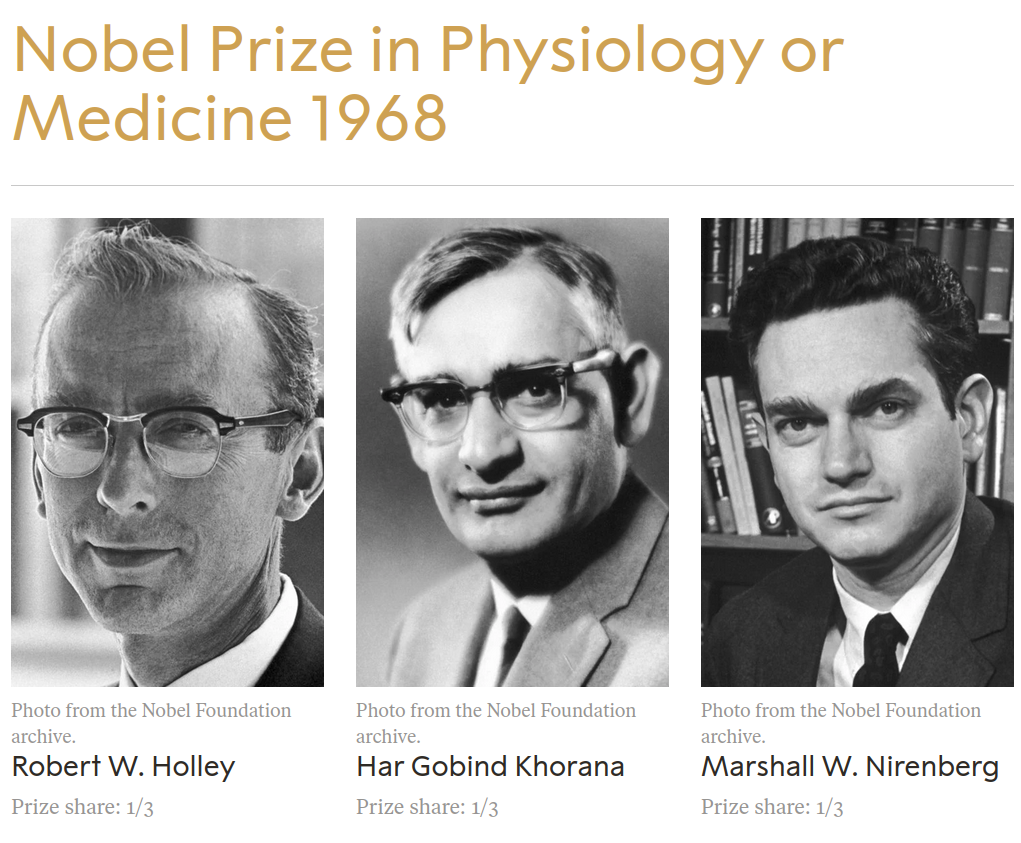
\includegraphics[width=\textwidth]{./figures/nobel1968.png}
		\end{figure}
		\column{0.5\textwidth}
		\begin{figure}
			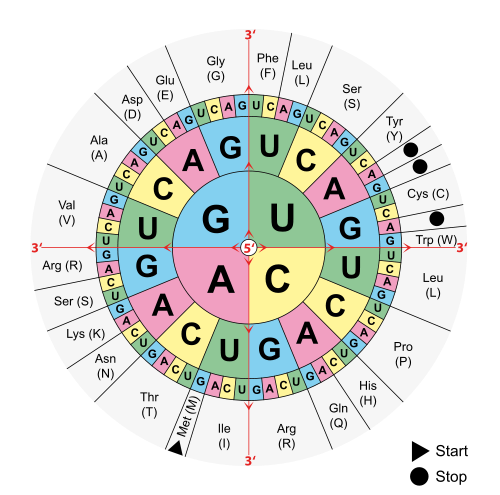
\includegraphics[width=\textwidth]{./figures/codesonne2.png}
		\end{figure}
	\end{columns}
	\begin{itemize}
		\item The genetic code is (almost) universal$^{[1]}$ 
		\item It was resolved entirely using synthetic sequences.
	\end{itemize}
	 \par {\scriptsize [1] http://www.ncbi.nlm.nih.gov/Taxonomy/taxonomyhome.html/index.cgi?chapter=tgencodes}
	\credit{https://www.nobelprize.org/prizes/medicine/1968/summary/ | User:Mouagip, Wikimedia Commons, PD}
\end{frame}

\begin{frame}{Encoded information of naturally occuring DNA unknown}
	\begin{columns}[T,onlytextwidth]
		\column{0.3\textwidth}
		\begin{figure}
			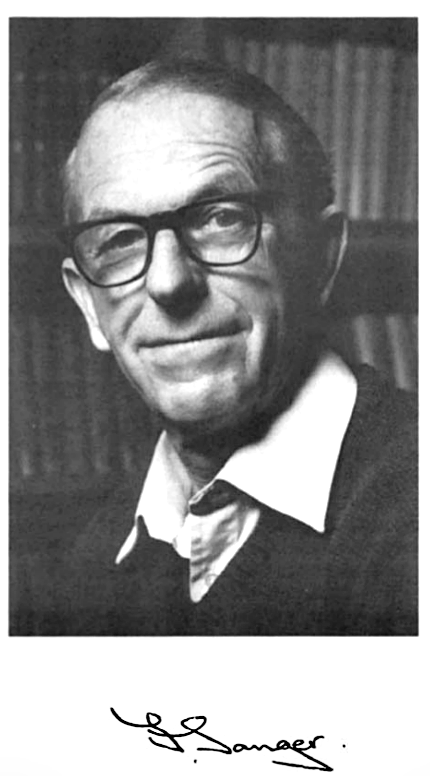
\includegraphics[width=\textwidth]{./figures/sanger.png}
		\end{figure}
		\column{0.7\textwidth}
		\vspace{3em}
		\begin{itemize}
			\item Peptides could be sequenced since the 
			1950s (Sanger method, Edman degradation).
			\item Sequencing of DNA was one of the most urgent, unresolved problems in the early 1970s.
			\item Frederick Sanger (Nobel laureate for sequencing Insulin 1958) started working with DNA. 
		\end{itemize}
	\end{columns}
\end{frame}

\begin{frame}{1977: Chain-termination sequencing by Frederick Sanger}
	\begin{columns}[T,onlytextwidth]
		\column{0.35\textwidth}
		\begin{figure}
			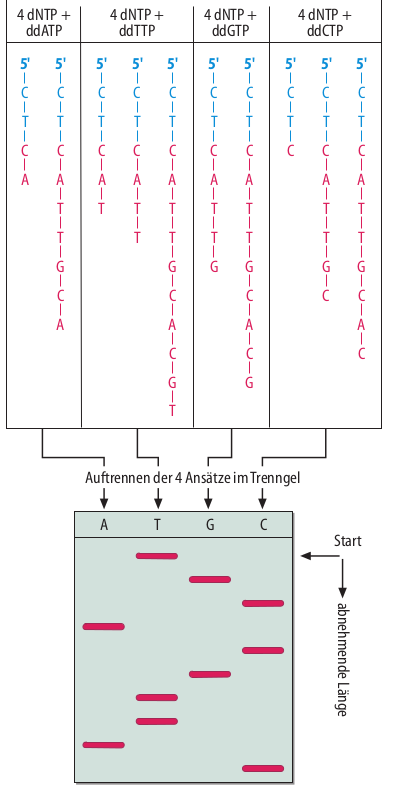
\includegraphics[width=\textwidth]{./figures/sangersequencing.png}
		\end{figure}
		\column{0.65\textwidth}
		\begin{itemize}
			\item DNA fragments could be separated by size.
			\item Sanger's method creates sequence-derived length patterns.
			\item It relies on radioactive labeling and in-vitro amplification of DNA.
		\end{itemize}
		\begin{figure}
			
\includegraphics[width=\textwidth]{./figures/sangerpaper.png}
			\caption{\citeme{Sanger1977}}
		\end{figure}
	\end{columns}
	\credit{$\leftarrow$ Fig.5.40, Löffler: Biochemie und Pathobiochemie 7th Ed.}
\end{frame}

\begin{frame}{1980: Nobel prize for DNA sequencing}
	\begin{columns}[T,onlytextwidth]
		\column{0.6\textwidth}
		\begin{figure}
			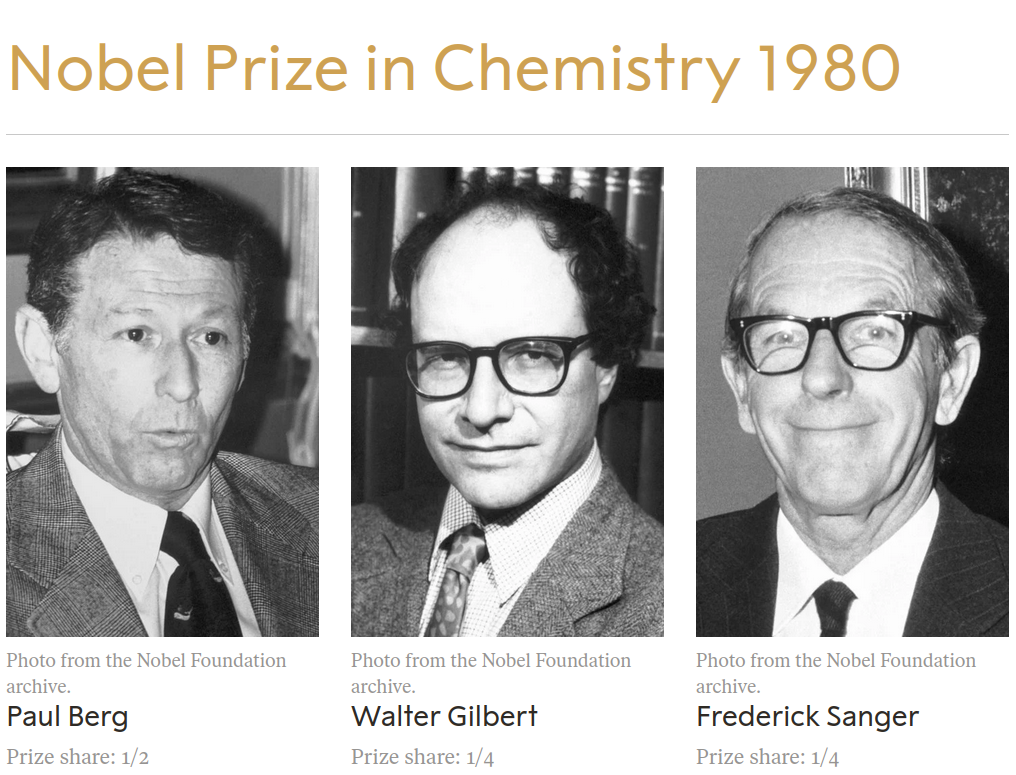
\includegraphics[width=\textwidth]{./figures/nobel-sanger.png}
		\end{figure}
		\column{0.5\textwidth}
		\begin{itemize}
			\item Ample DNA input needed\par {\scriptsize PCR was introduced in 1989}
			\item Four reactions per sequence
			\item Read length $\sim$ 200bp
		\end{itemize}
		\vspace{0.2cm}
		\begin{figure}
			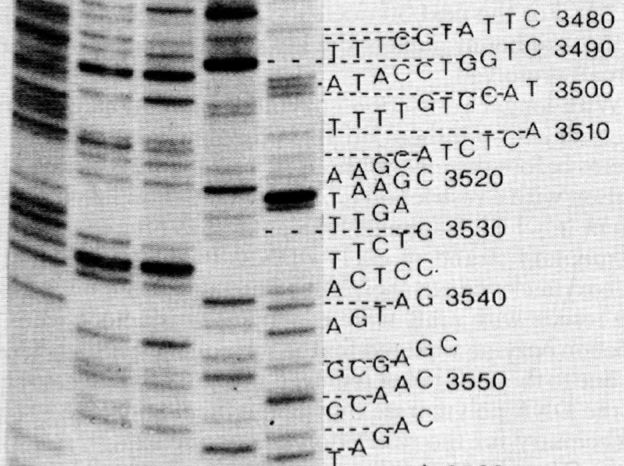
\includegraphics[width=0.8\textwidth]{./figures/sangergel.png}
		\end{figure}
	\end{columns}
 \creditleft{https://www.nobelprize.org/prizes/chemistry/1980/summary/}
\end{frame}

\begin{frame}{Advanced Sanger sequencing for the Human Genome Project}
	\begin{columns}[T,onlytextwidth]
		\column{0.5\textwidth}
		\begin{figure}
			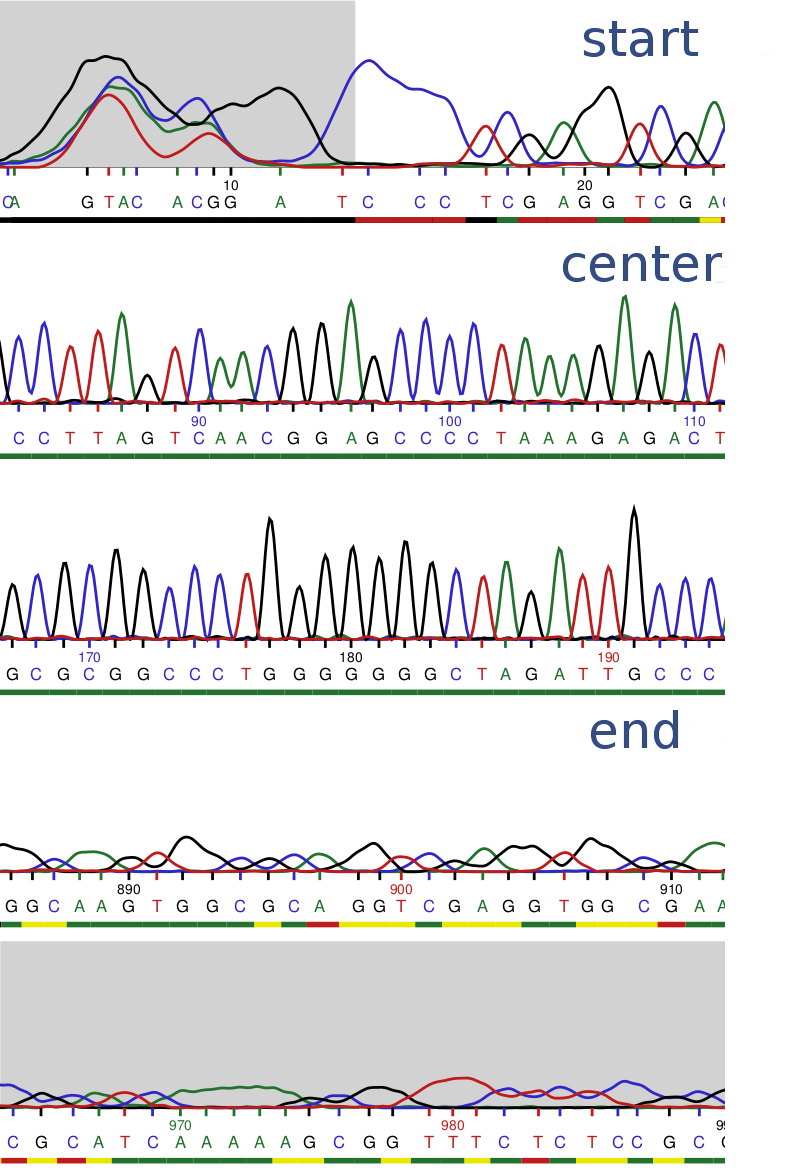
\includegraphics[width=\textwidth]{./figures/chromatogramm-eng.png}
		\end{figure}
		\column{0.5\textwidth}
		\begin{figure}
			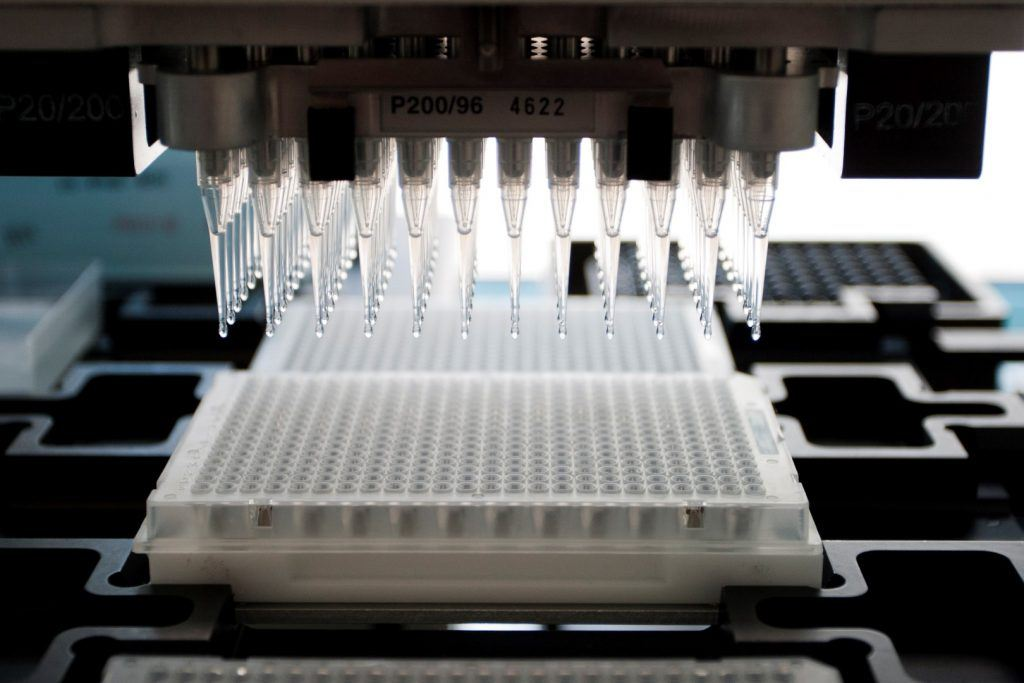
\includegraphics[width=\textwidth]{./figures/baseclearseq.jpg}
		\end{figure}
		\vspace{0.2cm}
		\begin{itemize}
			\item Fluorescent chain terminators.
			\item Capillary electrophoresis for size separation of amplicons.
			\item Parallelized and automated.
			\item Sequencing technology of the Human Genome Project (1990-2004).
		\end{itemize}
		\par \vspace{0.5cm}
		\credit{$\leftarrow$ A chromatogram generated by Sanger sequencing}
	\end{columns}
\end{frame}

% % % % % % % % % % % % % % % % % % % % % %  % % % % % % % % % %

\section{Next-generation sequencing}

% % % % % % % % % % % % % % % % % % % % % % % % % % % % % % % % % 

\begin{frame}{New high-throughput methods were developed}
	\begin{center}
		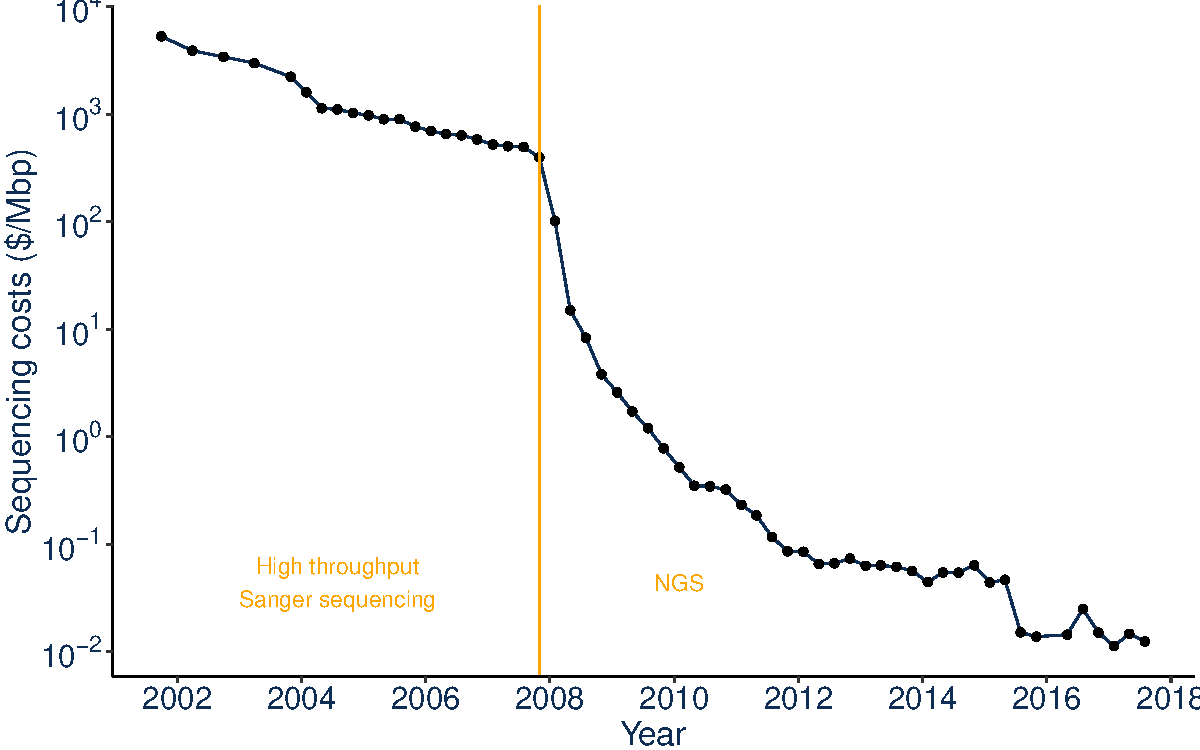
\includegraphics[width=0.9\textwidth]{./figures/sequencingcosts2018eng.pdf} \\
		Sequencing costs per one million bases of raw sequence
	\end{center}
	\credit{National Human Genome Research Institute (NHGRI), http://www.genome.gov/sequencingcosts}
\end{frame}

\begin{frame}{Sanger sequencing was outcompeted by NGS}
	\begin{columns}[T,onlytextwidth]
		\column{0.5\textwidth}
		\begin{figure}
			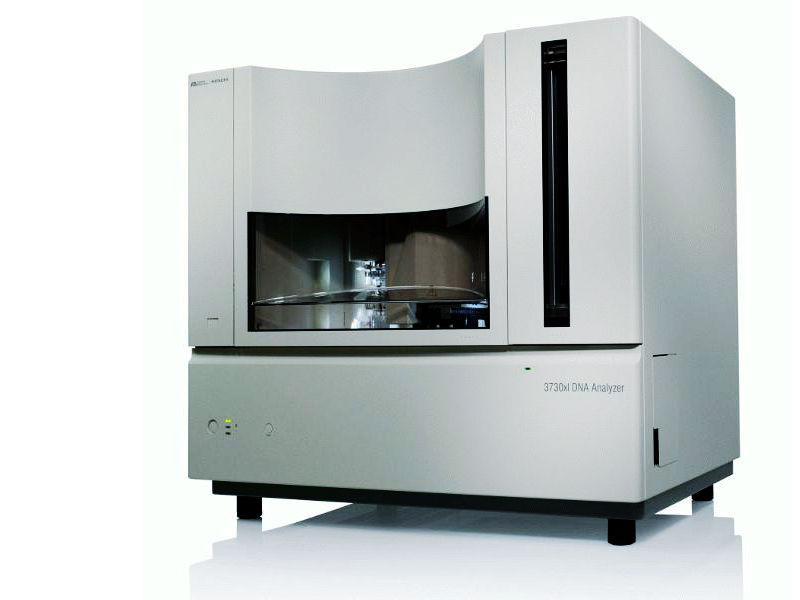
\includegraphics[width=0.8\textwidth]{./figures/abi3730xl.jpg} \vspace{1em} \\
		\end{figure}
		\column{0.5\textwidth}
		\begin{figure}
			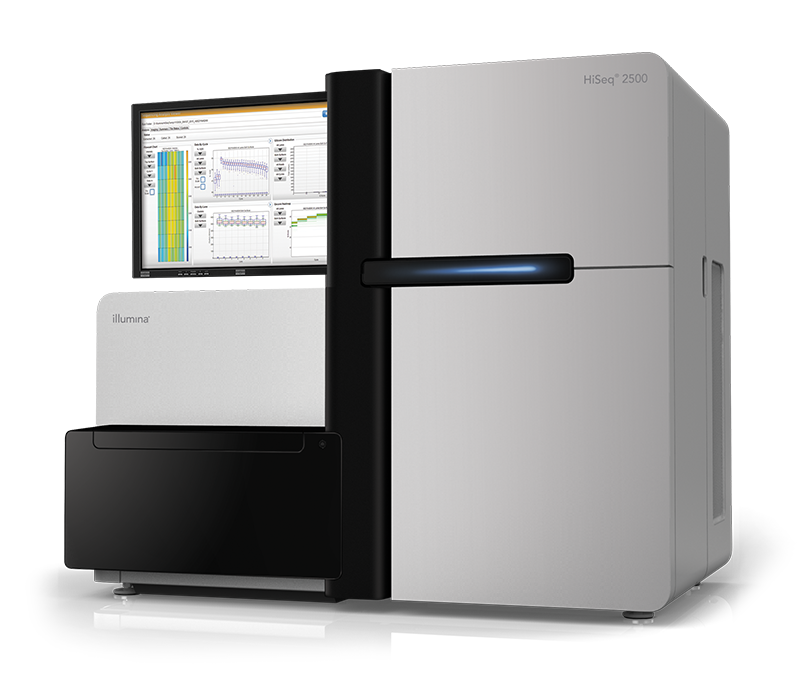
\includegraphics[width=0.8\textwidth]{./figures/system-carousel-hiseq2500-left.png}
		\end{figure}
	\end{columns}
	\begin{columns}[T,onlytextwidth]
		\column{0.5\textwidth}
		\begin{exampleblock}{}
			\textbf{ABI 3730xl DNA Sequencer}\\
			(Sanger Multiplex, 2013)
			\begin{itemize}
				\item $\sim$6912 reads of 400bp
				\item $\sim$2,76 Mbp / day
			\end{itemize}
		\end{exampleblock}
		\column{0.5\textwidth}
		\begin{exampleblock}{}
			\textbf{Illumina HiSeq 2500}  \vspace{0.3em} \\
			(NGS / MPS, 2013)
			\begin{itemize}
				\item $\sim$600 Million reads of 100bp
				\item $\sim$60.000 Mbp / day
			\end{itemize}
			{ \small (depending on settings and sequencing chemistry used)}
		\end{exampleblock}
	\end{columns}
\end{frame}

\section{References}
\begin{frame}[allowframebreaks]{References}
\begingroup
\renewcommand*{\bibfont}{\footnotesize} 
\printbibliography[heading=none]
\endgroup
\end{frame}

\end{document}
